\documentclass{article}
\usepackage[utf8]{inputenc}
\usepackage[spanish]{babel}
\usepackage{amsmath}
\usepackage{xcolor}
\usepackage{graphicx}

\graphicspath{{../../utils/}}

\begin{document}

\begin{titlepage}
    \centering
    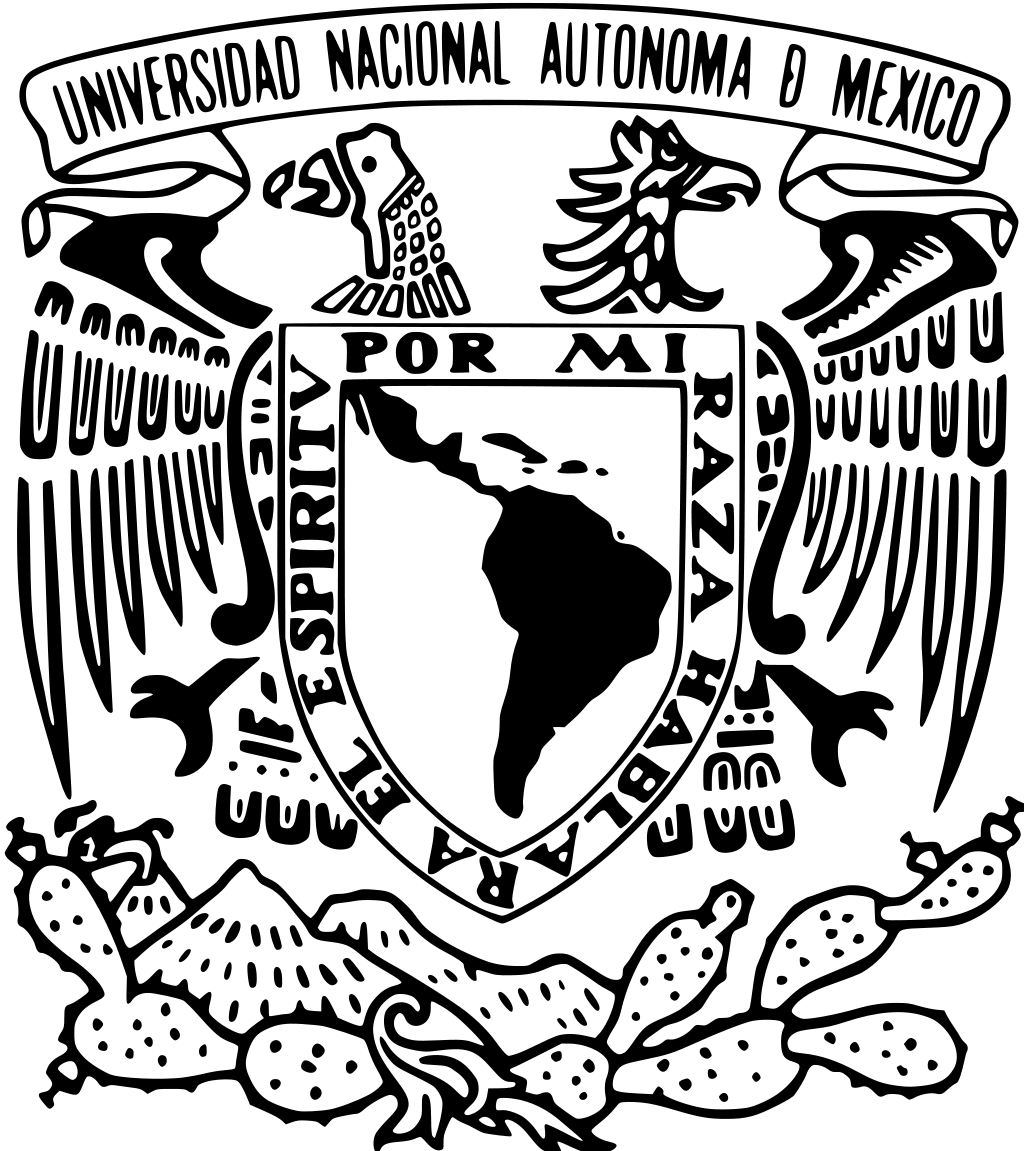
\includegraphics[width=0.50\textwidth]{unam_logo.png}\par
    \vspace{1cm}
    {\scshape\Large Universidad Nacional Autónoma de México \par}
    \vspace{1cm}
    {\scshape\Large Facultad de Ciencias \par}
    \vspace{1.5cm}
    {\huge\bfseries Arquitectura de Computadoras \par}
    {\huge\bfseries Tarea 1 \par}
    \vspace{2cm}
    {\Large\itshape David Rivera Morales\par}
    {\Large \itshape Christian Eulogio Sánchez \par}
    \vfill
  
\end{titlepage}



\section {Introducción}

Una \textbf{ALU (Unidad Aritmético-Lógica)} es un componente fundamental de un procesador o unidad de procesamiento central (CPU). Es el circuito digital encargado de realizar operaciones aritméticas y operaciones lógicas sobre los datos. Estas operaciones incluyen suma, resta, multiplicación, división, desplazamientos de bits, operaciones lógicas (\textit{AND, OR, XOR, NOT}), entre otras.

La ALU recibe los datos de entrada desde los registros del procesador, realiza la operación especificada por la unidad de control del procesador y almacena el resultado en otro registro. Es un componente crítico en el flujo de datos dentro del procesador y es responsable de ejecutar las instrucciones matemáticas y lógicas que forman parte de los programas de software.

Las ALUs modernas están diseñadas con circuitos integrados de alta velocidad y pueden manejar datos de diferentes tamaños, como 8, 16, 32 o 64 bits. Cuanto mayor sea el tamaño de la ALU, mayor será la capacidad de procesamiento de datos del procesador.

En resumen, la ALU es el ``cerebro'' aritmético y lógico de un procesador, encargada de realizar las operaciones fundamentales sobre los datos y permitiendo así la ejecución de programas y algoritmos complejos.




\section*{Preguntas}

    \section{¿Quién propuso por primera vez el diseño de una ALU? ¿Para qué computador se propuso?}
    \subsection*{Respuesta}
    \item La idea de una Unidad Aritmético-Lógica (ALU) fue propuesta por primera vez por John P. Eckert y John W. Mauchly en 1945 para la computadora ENIAC (Computadora Numérica Integrador y Calculadora).

    \section{¿Qué es VHDL? ¿Cómo se ve un full-adder en VHDL?}
    \subsection*{Respuesta}
    \item VHDL (Lenguaje de Descripción de Hardware de Muy Alto Nivel) es un lenguaje de programación utilizado para describir circuitos digitales y sistemas embebidos. Un ejemplo de un sumador completo (full-adder) en VHDL sería:

    \begin{verbatim}
    library IEEE;
    use IEEE.STD_LOGIC_1164.ALL;

    entity full_adder is
        Port ( a, b, cin : in STD_LOGIC;
              sum, cout : out STD_LOGIC);
    end full_adder;

    architecture Behavioral of full_adder is
    begin
        sum <= a xor b xor cin;
        cout <= (a and b) or (a and cin) or (b and cin);
    end Behavioral;
    \end{verbatim}

    \section{¿Qué operaciones aritméticas y lógicas son básicas para un procesador? Justifica tu respuesta.}
    \subsection*{Respuesta}
    \item Las operaciones aritméticas y lógicas básicas para un procesador son la suma, resta, multiplicación, división, operaciones lógicas (AND, OR, NOT, XOR), y desplazamientos de bits. Estas operaciones son fundamentales para realizar cálculos numéricos, manipular datos y controlar el flujo de ejecución del programa.


    \section{El diseño utilizado para realizar la adición resulta ser ineficiente, ¿por qué? ¿Qué tipo de sumador resulta ser más eficiente?}
    \subsection*{Respuesta}
    \item El diseño utilizado para realizar la adición resulta ineficiente debido a la propagación de acarreo (carry). En un sumador de varios bits, el acarreo generado en un bit debe propagarse a los bits superiores, lo que aumenta el tiempo de cálculo. Un sumador más eficiente es el sumador de propagación de acarreo (carry-lookahead adder), que utiliza circuitos adicionales para calcular el acarreo en paralelo, reduciendo el tiempo de cálculo.

  

    \section{Bajo este diseño, en la ALU se calculan todas las operaciones de forma simultánea pero solo se entrega un resultado, ¿se realiza trabajo inútil? ¿Toma tiempo adicional? ¿Cuál es el costo?}
    \subsection*{Respuesta}
    \item En el diseño de la ALU donde se calculan todas las operaciones de forma simultánea pero solo se entrega un resultado, se realiza trabajo inútil ya que solo una de las operaciones es utilizada en un momento dado. Esto consume tiempo adicional y energía, lo que aumenta el costo en términos de rendimiento y consumo de energía.


    \section{¿Cuántas operaciones más podemos agregar al diseño de esta ALU? ¿Qué tendríamos que modificar para realizar más operaciones?}
    \subsection*{Respuesta}
    \item En teoría, se pueden agregar más operaciones al diseño de la ALU, pero esto implica agregar más circuitos lógicos y aumentar la complejidad del diseño. Para realizar más operaciones, se tendría que modificar la lógica de control de la ALU, así como los circuitos de operación correspondientes.


\end{document}
